% Taxonomy of non-market valuation methods.
% Compile to SVG:  latex valuation_methods.tex && dvisvgm --no-fonts valuation_methods.dvi -o ../valuation_methods.svg
\documentclass[tikz,border=6pt]{standalone}
\usepackage[scaled]{helvet}
\renewcommand{\familydefault}{\sfdefault}
\usetikzlibrary{positioning}
\definecolor{blu}{HTML}{3B6EA8}
\definecolor{accent}{HTML}{2E7D32}
\begin{document}
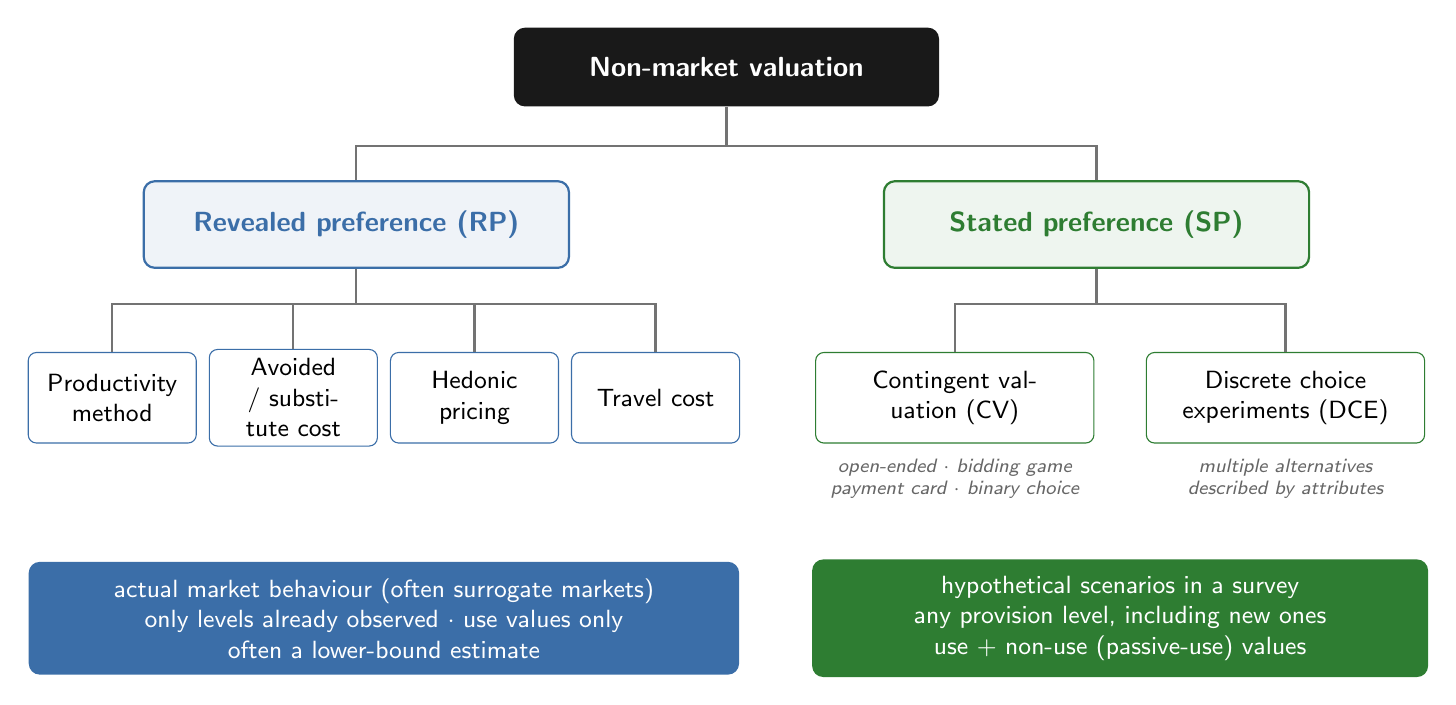
\begin{tikzpicture}[
    edge/.style={draw=black!55, thick},
    root/.style={fill=black!90, text=white, font=\bfseries, rounded corners=4pt,
                 minimum width=5.4cm, minimum height=1cm},
    fam/.style={draw=#1, fill=#1!8, text=#1, thick, font=\bfseries, rounded corners=4pt,
                minimum width=5.4cm, minimum height=1.1cm},
    meth/.style={draw=#1, fill=white, rounded corners=3pt, align=center, font=\small,
                 minimum height=1.15cm, text width=1.9cm},
    smeth/.style={meth=#1, text width=3.3cm},
    note/.style={font=\scriptsize\itshape, text=black!60, align=center},
    prop/.style={fill=#1, text=white, rounded corners=4pt, align=center, font=\small,
                 inner sep=6pt}]
  \node[root] (root) at (0,0) {Non-market valuation};
  \node[fam=blu]    (rp) at (-4.7,-2) {Revealed preference (RP)};
  \node[fam=accent] (sp) at ( 4.7,-2) {Stated preference (SP)};
  \node[meth=blu] (m1) at (-7.8,-4.2) {Productivity method};
  \node[meth=blu] (m2) at (-5.5,-4.2) {Avoided / substitute cost};
  \node[meth=blu] (m3) at (-3.2,-4.2) {Hedonic pricing};
  \node[meth=blu] (m4) at (-0.9,-4.2) {Travel cost};
  \node[smeth=accent] (cv)  at (2.9,-4.2) {Contingent valuation (CV)};
  \node[smeth=accent] (dce) at (7.1,-4.2) {Discrete choice experiments (DCE)};
  \node[note, below=2pt of cv]  {open-ended $\cdot$ bidding game\\payment card $\cdot$ binary choice};
  \node[note, below=2pt of dce] {multiple alternatives\\described by attributes};
  \draw[edge] (root.south) -- ++(0,-0.5) -| (rp.north);
  \draw[edge] (root.south) -- ++(0,-0.5) -| (sp.north);
  \foreach \m in {m1,m2,m3,m4} \draw[edge] (rp.south) -- ++(0,-0.45) -| (\m.north);
  \foreach \m in {cv,dce}       \draw[edge] (sp.south) -- ++(0,-0.45) -| (\m.north);
  \node[prop=blu, text width=8.6cm] at (-4.35,-7)
    {actual market behaviour (often surrogate markets)\\only levels already observed $\cdot$ use values only\\often a lower-bound estimate};
  \node[prop=accent, text width=7.4cm] at (5,-7)
    {hypothetical scenarios in a survey\\any provision level, including new ones\\use + non-use (passive-use) values};
\end{tikzpicture}
\end{document}
